\documentclass[mathserif,spanish,10pt]{beamer}

\mode<presentation>{
  \usetheme{Madrid}
  \usecolortheme{whale}
  \setbeamertemplate{footline}[frame number]
  \setbeamertemplate{navigation symbols}{}
}

\usepackage{graphicx}
\usepackage{booktabs}
\usepackage{multirow}
\usepackage{caption}
\usepackage{subcaption}
\usefonttheme{professionalfonts}
\usepackage{ragged2e}
\justifying
\usepackage[utf8]{inputenc}
\usepackage[spanish]{babel}
\makeatletter
\AtBeginDocument{\def\%{\@percentchar}}
\makeatother
\usepackage{amsmath}
\usepackage{mathtools}
\usepackage{xcolor}
\usepackage{colortbl}
\usepackage{array}
\usepackage{tikz}
\usetikzlibrary{shapes,arrows,positioning}

% ── Colores ──────────────────────────────────────────────────────────────────
\definecolor{navyblue}{RGB}{13,31,78}
\definecolor{accentteal}{RGB}{8,145,178}
\definecolor{lightblue}{RGB}{186,230,253}
\definecolor{kpigreen}{RGB}{22,163,74}
\definecolor{kpiorange}{RGB}{234,88,12}
\definecolor{rowsim}{RGB}{239,246,255}
\definecolor{rowexp}{RGB}{240,253,244}
\definecolor{rowhdr}{RGB}{13,31,78}
\definecolor{passgreen}{RGB}{22,163,74}
\definecolor{failred}{RGB}{220,38,38}

\newcommand{\highlight}[1]{\textbf{\color{accentteal}#1}}
\newcommand{\good}[1]{\textcolor{passgreen}{#1}}
\newcommand{\bad}[1]{\textcolor{failred}{#1}}
\newcommand{\warn}[1]{\textbf{\color{kpiorange}#1}}
\newcommand{\pass}{\good{\checkmark}}
\newcommand{\fail}{\bad{$\times$}}

\captionsetup{font=scriptsize,labelfont=bf,labelsep=period,justification=centering}

% ── Metadatos ────────────────────────────────────────────────────────────────
\title[Lab~4 · Heli~2DoF]{Identificación y Control del Helicóptero de Dos Grados de Libertad}
\subtitle{Grupo~B --- Laboratorio de Control Automático}
\author[Castro, Chavarría, Segura]{E.\,Castro \and D.\,Chavarría \and E.\,Segura}
\institute[TEC]{Instituto Tecnológico de Costa Rica \\ Escuela de Ingeniería Electrónica}
\date{\today}

% ════════════════════════════════════════════════════════════════════════════
\begin{document}

% ── Portada ──────────────────────────────────────────────────────────────────
\begin{frame}[plain]
  \titlepage
\end{frame}

% ── Tabla de contenidos ──────────────────────────────────────────────────────
\begin{frame}{Contenido}
  \tableofcontents[sectionstyle=show,subsectionstyle=show/shaded/hide]
\end{frame}

\AtBeginSection[]{
  \begin{frame}{Contenido}
    \tableofcontents[currentsection,sectionstyle=show/shaded,subsectionstyle=show/shaded/hide]
  \end{frame}
}

%=============================================================================
\section{Objetivo}
%=============================================================================

\begin{frame}{Objetivo}
\begin{columns}[T]
  \column{0.55\textwidth}
  \begin{block}{Metas del laboratorio}
    \begin{itemize}
      \item Identificar experimentalmente la planta Heli~2DoF (MIMO~2$\times$2).
      \item Construir modelo en espacio de estados a partir de funciones SISO.
      \item Diseñar y evaluar controladores \textbf{REI} (Regulador con Estado Integral):
        \begin{itemize}
          \item \textit{Pole Placement} (PP)
          \item Regulador Lineal Cuadrático (LQR)
        \end{itemize}
      \item Validar en simulación y verificar experimentalmente.
    \end{itemize}
  \end{block}

  \column{0.42\textwidth}
  \begin{block}{Especificaciones de diseño}
    \vspace{0.2cm}
    \centering\small
    \rowcolors{2}{rowsim}{white}
    \begin{tabular}{cl}
      \hline
      \rowcolor{rowhdr}
      \color{white}\textbf{Métrica} & \color{white}\textbf{Límite} \\
      \hline
      $t_{s_{2\%}}$ & $< 8\,\text{s}$ \\[3pt]
      $M_p$         & $< 5\,\%$ \\[3pt]
      $e_{ss}$      & $< 0.003\,\text{rad}$ \\[3pt]
      $|\beta|_{\max}$ & $< 0.1\,\text{rad}$ \\
      \hline
    \end{tabular}
  \end{block}
\end{columns}
\end{frame}

%=============================================================================
\section{Planta y Descripción del Sistema}
%=============================================================================

\begin{frame}{Planta Heli~2DoF}
\begin{columns}[T]
  \column{0.54\textwidth}
  \begin{block}{Descripción física}
    \begin{itemize}
      \item Brazo de aluminio sobre eje central fijo a base de madera.
      \item Dos motores DC (24\,V, brushed) + hélices GEMFAN 5045BN.
      \item Encoders ópticos USDigital E5 (900\,PPR, 3600\,CPR).
      \item Constante angular: $k_\theta = 2\pi/3600 = 0.001745\,\text{rad/cnt}$.
      \item PWM: $T_{pwm}=500\,\mu\text{s}$, amplitud 24\,V.
      \item Periodo de muestreo: $T_s = 20\,\text{ms}$.
      \item Enlace Bluetooth para encoder de pitch.
    \end{itemize}
  \end{block}

  \column{0.42\textwidth}
  \begin{block}{Variables del sistema}
    \centering\small
    \rowcolors{2}{rowsim}{white}
    \begin{tabular}{cl}
      \hline
      \rowcolor{rowhdr}
      \color{white}\textbf{Símbolo} & \color{white}\textbf{Descripción} \\
      \hline
      $\theta$      & Ángulo de pitch \\[3pt]
      $\beta$       & Ángulo de yaw \\[3pt]
      $e_p$         & Voltaje motor pitch \\[3pt]
      $e_y$         & Voltaje motor yaw \\[3pt]
      \hline
    \end{tabular}
  \end{block}

  \begin{block}{Estructura MIMO}
    \centering\small
    $\mathbf{u} = [e_p,\; e_y]^T$\quad
    $\mathbf{y} = [\theta,\; \beta]^T$
  \end{block}
\end{columns}
\end{frame}

%=============================================================================
\section{Identificación del Sistema}
%=============================================================================

\subsection{Protocolo experimental}

\begin{frame}{Protocolo de Identificación}
\begin{columns}[T]
  \column{0.50\textwidth}
  \begin{block}{Experimento de Pitch}
    \begin{itemize}
      \item Perfil trapezoidal hasta 18.7\,V al motor de pitch desde $t=1\,\text{s}$.
      \item Pulso rectangular 6\,V al yaw ($t=12$--$20\,\text{s}$) para contrarrestar drift.
      \item Se registran $\theta(t)$ y $\beta(t)$.
      \item Datos usados: primeros $10\,\text{s}$ para PITCH, primeros $4\,\text{s}$ para canal cruzado.
    \end{itemize}
  \end{block}

  \begin{block}{Experimento de Yaw}
    \begin{itemize}
      \item Pulso 6\,V al motor de yaw ($t=1$--$20\,\text{s}$), motor pitch apagado.
      \item Se registra $\beta(t)$.
      \item Datos usados: primeros $4\,\text{s}$.
    \end{itemize}
  \end{block}

  \column{0.46\textwidth}
  \begin{block}{Procesamiento (MATLAB \texttt{ident})}
    \begin{itemize}
      \item Eliminación de entradas de tiempo negativo.
      \item Ajuste de funciones de transferencia SISO para cada canal.
      \item Acoplamiento yaw$\to$pitch despreciable: $G_{21}(s)\approx 0$.
    \end{itemize}
  \end{block}

  \begin{alertblock}{Sistema identificado}
    \centering
    $4$ canales SISO $\to$ modelo MIMO $2\times2$
  \end{alertblock}
\end{columns}
\end{frame}

%─────────────────────────────────────────────────────────────────────────────
\subsection{Modelos SISO y parámetros}

\begin{frame}{Modelos SISO Identificados}
\begin{columns}[T]
  \column{0.50\textwidth}
  \begin{block}{Canal Pitch $\theta/e_p$}
    \[
      G_{11}(s) = \frac{k_p(s + z_p)}{s^2 + a_{1p}s + a_{0p}}
    \]
  \end{block}
  \vspace{-4pt}
  \begin{block}{Canal Yaw $\beta/e_y$}
    \[
      G_{22}(s) = \frac{-k_y}{s(s + p_y)}
    \]
  \end{block}
  \vspace{-4pt}
  \begin{block}{Acoplamiento $\beta/e_p$}
    \[
      G_{21}(s) = \frac{k_{yp}}{s}, \quad G_{12}(s)\approx 0
    \]
  \end{block}

  \column{0.46\textwidth}
  \begin{table}
    \centering
    \caption{Parámetros identificados.}
    \scriptsize
    \rowcolors{2}{rowsim}{white}
    \begin{tabular}{lcc}
      \hline
      \rowcolor{rowhdr}
      \color{white}\textbf{Parámetro} &
      \color{white}\textbf{Símbolo} &
      \color{white}\textbf{Valor} \\
      \hline
      Ganancia pitch  & $k_p$    & 0.01462  \\
      Cero pitch      & $z_p$    & 3.9330   \\
      Amort.\ pitch   & $a_{1p}$ & 0.4450   \\
      Frec.\ pitch    & $a_{0p}$ & 1.6410   \\
      Ganancia yaw    & $k_y$    & 0.03164  \\
      Polo yaw        & $p_y$    & 0.1000   \\
      Acoplamiento    & $k_{yp}$ & 0.1600   \\
      \hline
    \end{tabular}
  \end{table}
\end{columns}
\end{frame}

%─────────────────────────────────────────────────────────────────────────────
\subsection{Modelo MIMO en espacio de estados}

\begin{frame}{Modelo MIMO en Espacio de Estados}
\begin{columns}[T]
  \column{0.55\textwidth}
  \vspace{-4pt}
  \[
    \mathbf{x}^T = \begin{bmatrix} \theta & \beta & \dot\theta & \dot\beta \end{bmatrix}
  \]
  \[
    A = \begin{bmatrix}
          0 & 0 & 1 & 0 \\
          0 & 0 & 0 & 1 \\
          -1.641 & 0 & -0.445 & 0 \\
          0 & 0 & 0 & -0.1
        \end{bmatrix}
  \]
  \[
    B = \begin{bmatrix}
          k_p & 0 \\
          k_{yp} & 0 \\
          k_p z_p & 0 \\
          0 & -k_y
        \end{bmatrix}, \quad
    C = \begin{bmatrix}1&0&0&0\\0&1&0&0\end{bmatrix}
  \]

  \column{0.41\textwidth}
  \begin{block}{Observaciones clave}
    \scriptsize
    \begin{itemize}
      \item Sistema de \textbf{4.º orden}: estado $[\theta,\beta,\dot\theta,\dot\beta]$.
      \item Forma canónica observable (OCF).
      \item Acoplamiento $k_{yp}$: pitch afecta yaw.
      \item Canal yaw $\approx$ integrador (polo $p_y=0.1$ lento).
    \end{itemize}
  \end{block}

  \begin{block}{Verificación}
    \centering\small
    Recuperación de las 4 FT SISO con\\
    \texttt{zpk(modeloHeli)} en MATLAB. \good{$\checkmark$}
  \end{block}
\end{columns}
\end{frame}

%=============================================================================
\section{Diseño de Controladores REI}
%=============================================================================

\begin{frame}{Estructura del Regulador con Estado Integral (REI)}
\begin{columns}[T]
  \column{0.52\textwidth}
  \begin{block}{Ley de control}
    \begin{itemize}
      \item Estado aumentado: $\mathbf{x}_e^T = [\mathbf{x}^T\;\; \mathbf{x}_I^T]$
      \item $\dot{\mathbf{x}}_I = \mathbf{r} - \mathbf{y}$ \quad (error integrado)
      \item Control: $\mathbf{u} = -\mathbf{K}\mathbf{x} - \mathbf{K}_i\mathbf{x}_I$
      \item Sistema aumentado: \textbf{6 polos} ($4+2$ integradores).
    \end{itemize}
  \end{block}
  \begin{block}{Beneficios}
    \scriptsize
    \begin{itemize}
      \item $e_{ss}=0$ garantizado ante escalón.
      \item Supresión activa de perturbaciones.
      \item Control MIMO desacoplado pitch/yaw.
    \end{itemize}
  \end{block}

  \column{0.44\textwidth}
  \begin{block}{Técnicas evaluadas}
    \centering\small
    \vspace{4pt}
    \rowcolors{2}{rowsim}{white}
    \begin{tabular}{p{1.5cm}p{2.2cm}}
      \rowcolor{rowhdr}
      \color{white}\textbf{Método} & \color{white}\textbf{Criterio} \\
      Pole Placement & Polos dominantes deseados \\
      LQR & Minimización del costo $J$ \\
    \end{tabular}
    \vspace{6pt}
  \end{block}
  \begin{alertblock}{Referencia (Simulink)}
    \centering
    $[\theta_r;\,\beta_r]=[0.583;\,0]\,\text{rad}$
  \end{alertblock}
\end{columns}
\end{frame}

%─────────────────────────────────────────────────────────────────────────────
\subsection{Pole Placement}

\begin{frame}{Pole Placement --- Diseño}
\begin{columns}[T]
  \column{0.50\textwidth}
  \begin{block}{Metodología}
    \begin{enumerate}
      \item Sistema aumentado ($4+2=6$ estados).
      \item Par dominante: satisfacer $t_s$ y $M_p$.
      \item Polos rápidos: parte real $\geq 5\times$ la del par dominante.
      \item Cálculo: \texttt{place(Ae,Be,p)} en MATLAB.
    \end{enumerate}
  \end{block}

  \begin{block}{Ganancias obtenidas}
    \centering\scriptsize
    \[
      \mathbf{K}_{PP} = \begin{bmatrix}
        56.61 & -17.84 & 2.28 & -0.82
      \end{bmatrix}
    \]
    \[
      \mathbf{K}_{i,PP} = \begin{bmatrix} 35.47 & 0 \\ 0 & (\cdot) \end{bmatrix}
    \]
  \end{block}

  \column{0.46\textwidth}
  \begin{block}{Polos en lazo cerrado}
    \centering\small
    \[
    \begin{split}
      \lambda^{PP} = \{ & \underbrace{-1.08\pm j0.97}_{\text{dominantes}},\\
                        & -4.32,\;-5.40,\;-6.49 \}
    \end{split}
    \]
  \end{block}

  \begin{block}{Especificaciones esperadas}
    \centering\scriptsize
    Par dominante: $\zeta\approx0.745$\\
    $t_{s_{2\%}}\approx\dfrac{4}{\zeta\omega_n} \approx 3.7\,\text{s}$\\
    $M_p \approx 2.5\,\%$
  \end{block}
\end{columns}
\end{frame}

%─────────────────────────────────────────────────────────────────────────────
\begin{frame}{Pole Placement --- Resultados: Pitch}
\begin{columns}[T]

  \column{0.48\textwidth}
  {\centering\small\color{navyblue}\textbf{Simulación}\par}
  \vspace{4pt}
  \begin{center}
    \fbox{\parbox{0.88\linewidth}{\centering\vspace{1.8cm}
    {\scriptsize [Figura: Respuesta pitch PP simulación]}\vspace{1.8cm}}}
  \end{center}
  \vspace{-4pt}
  \begin{table}
    \centering\scriptsize
    \rowcolors{2}{rowsim}{white}
    \begin{tabular}{lcc}
      \hline
      \rowcolor{rowhdr}
      \color{white}\textbf{Métrica} & \color{white}\textbf{Valor} & \color{white}\textbf{Espec.} \\
      \hline
      $t_s$ (s)  & 4.4995 & $<8$ \pass \\
      $M_p$ (\%) & 2.4194 & $<5$ \pass \\
      $e_{ss}$ (rad) & 0 & $<0.003$ \pass \\
      \hline
    \end{tabular}
  \end{table}

  \column{0.48\textwidth}
  {\centering\small\color{navyblue}\textbf{Experimento (Self-Checker)}\par}
  \vspace{4pt}
  \begin{center}
    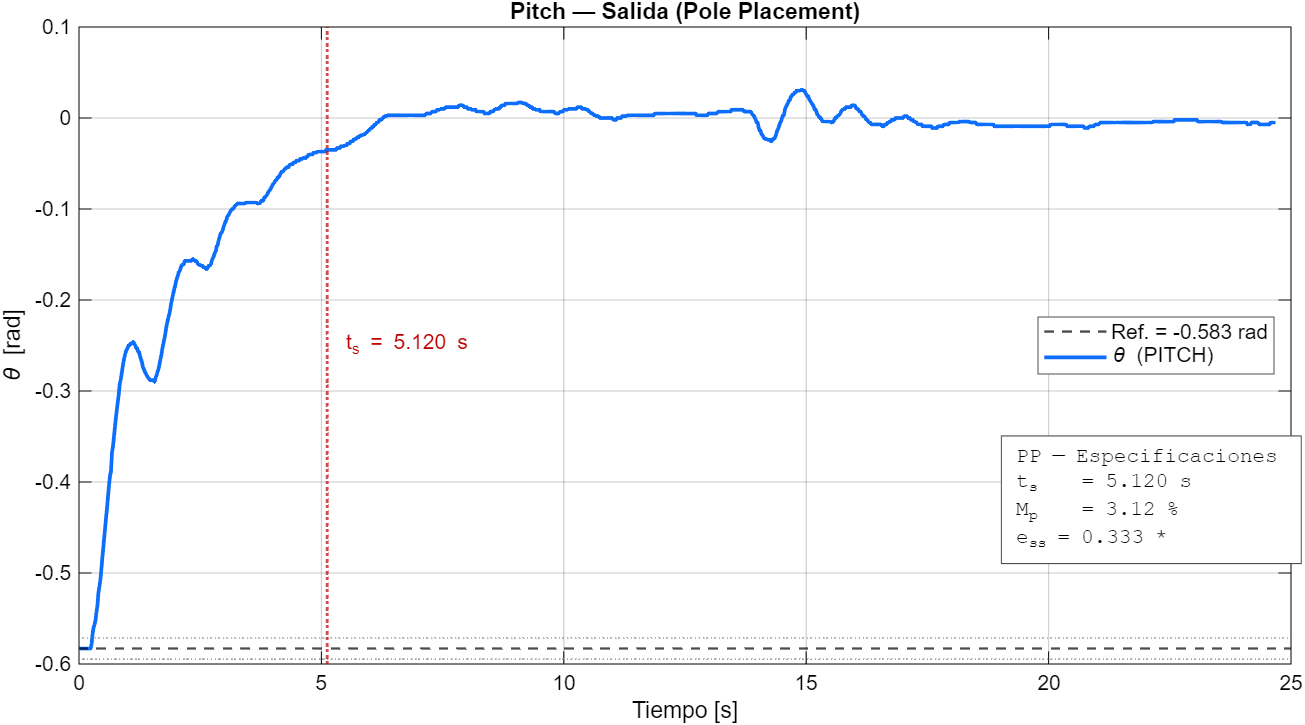
\includegraphics[width=0.95\linewidth,height=3.6cm,keepaspectratio]{PP_Pitch.png}
  \end{center}
  \vspace{-4pt}
  \begin{table}
    \centering\scriptsize
    \rowcolors{2}{rowexp}{white}
    \begin{tabular}{lcc}
      \hline
      \rowcolor{rowhdr}
      \color{white}\textbf{Métrica} & \color{white}\textbf{Valor} & \color{white}\textbf{Espec.} \\
      \hline
      $t_s$ (s)  & 5.120 & $<8$ \pass \\
      $M_p$ (\%) & 3.12  & $<5$ \pass \\
      $e_{ss}$ (IAE) & 0.333 & $<0.003$ \bad{---} \\
      \hline
    \end{tabular}
  \end{table}

\end{columns}
\end{frame}

%─────────────────────────────────────────────────────────────────────────────
\begin{frame}{Pole Placement --- Resultados: Yaw \& Perturbación}
\begin{columns}[T]

  \column{0.48\textwidth}
  {\centering\small\color{navyblue}\textbf{Restricción Yaw}\par}
  \vspace{4pt}
  \begin{center}
    \includegraphics[width=0.95\linewidth,height=3.6cm,keepaspectratio]{PP_Yaw.png}
  \end{center}
  \vspace{-4pt}
  \begin{table}
    \centering\scriptsize
    \rowcolors{2}{rowexp}{white}
    \begin{tabular}{lcc}
      \hline
      \rowcolor{rowhdr}
      \color{white}\textbf{Métrica} & \color{white}\textbf{Valor} & \color{white}\textbf{Espec.} \\
      \hline
      $|\beta|_{\max}$ (rad) & 0.1010 & $<0.1$ \warn{$\approx$} \\
      Nota SC & 99.0/100 & --- \\
      \hline
    \end{tabular}
  \end{table}
  {\centering\fontsize{7pt}{8pt}\selectfont
  Constraint parcial: $0.1010\in(0.1,0.2)$\par}

  \column{0.48\textwidth}
  {\centering\small\color{navyblue}\textbf{Rechazo de Perturbación}\par}
  \vspace{4pt}
  \begin{center}
    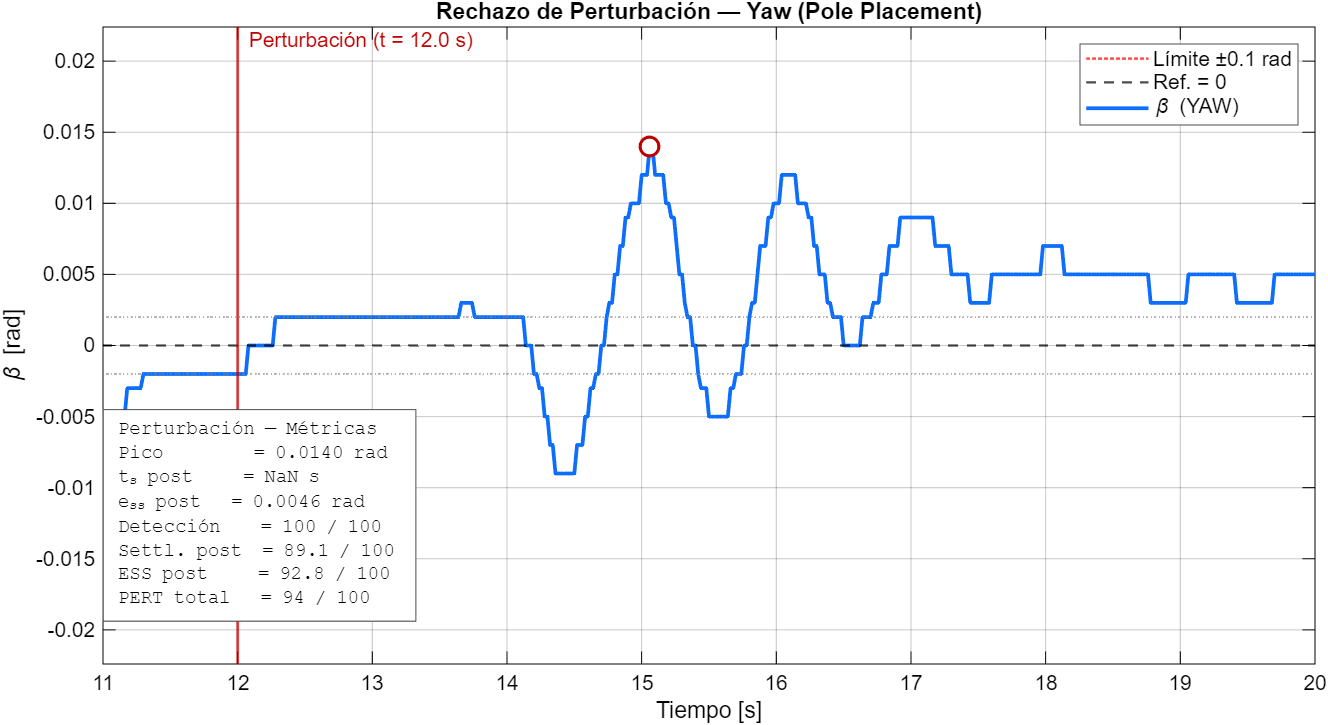
\includegraphics[width=0.95\linewidth,height=3.6cm,keepaspectratio]{PP_Pert_Yaw.png}
  \end{center}
  \vspace{-4pt}
  \begin{table}
    \centering\scriptsize
    \rowcolors{2}{rowexp}{white}
    \begin{tabular}{lc}
      \hline
      \rowcolor{rowhdr}
      \color{white}\textbf{Componente SC} & \color{white}\textbf{Puntos} \\
      \hline
      Detección      & 100/100 \\
      Settling post  & 89.1/100 \\
      ESS post       & 92.8/100 \\
      \textbf{PERT total} & \textbf{94/100} \\
      \hline
    \end{tabular}
  \end{table}

\end{columns}
\end{frame}

%─────────────────────────────────────────────────────────────────────────────
\subsection{LQR}

\begin{frame}{LQR --- Diseño}
\begin{columns}[T]
  \column{0.50\textwidth}
  \begin{block}{Función de costo}
    \[
      J = \int_0^\infty \!\left(\mathbf{x}_e^T\mathbf{Q}\mathbf{x}_e + \mathbf{u}^T\mathbf{R}\mathbf{u}\right)dt
    \]
  \end{block}

  \vspace{4pt}
  \begin{block}{Ganancias óptimas}
    \centering\scriptsize
    \[
      \mathbf{K} = \begin{bmatrix}
        27.76 & 2.89 & 16.21 & 1.15 \\
        2.76 & -53.25 & 2.98 & -41.78
      \end{bmatrix}
    \]
    \[
      \mathbf{K}_i = \begin{bmatrix}
        25.83 & 2.09 \\
        5.90 & -30.20
      \end{bmatrix}
    \]
  \end{block}

  \column{0.46\textwidth}
  \begin{table}
    \centering
    \caption{Pesos $\mathbf{Q}$ y $\mathbf{R}$ (ajuste iterativo).}
    \scriptsize
    \rowcolors{2}{rowsim}{white}
    \begin{tabular}{p{1.6cm}cc}
      \rowcolor{rowhdr}
      \color{white}\textbf{Estado} &
      \color{white}$Q_{ii}$ & \\
      \midrule
      $\theta$         & ajustado \\
      $\beta$          & ajustado \\
      $\dot\theta$     & ajustado \\
      $\dot\beta$      & ajustado \\
      $x_{I,\theta}$   & ajustado \\
      $x_{I,\beta}$    & ajustado \\
      \multicolumn{2}{l}{$\mathbf{R}$: penalización control}\\
    \end{tabular}
  \end{table}

  \begin{alertblock}{Criterio de ajuste}
    \centering\scriptsize
    Iteración hasta cumplir\\
    $t_s<8\,\text{s}$, $M_p<5\%$, $|\beta|<0.1\,\text{rad}$
  \end{alertblock}
\end{columns}
\end{frame}

%─────────────────────────────────────────────────────────────────────────────
\begin{frame}{LQR --- Resultados: Pitch}
\begin{columns}[T]

  \column{0.48\textwidth}
  {\centering\small\color{navyblue}\textbf{Simulación}\par}
  \vspace{4pt}
  \begin{center}
    \fbox{\parbox{0.88\linewidth}{\centering\vspace{1.8cm}
    {\scriptsize [Figura: Respuesta pitch LQR simulación]}\vspace{1.8cm}}}
  \end{center}
  \vspace{-4pt}
  \begin{table}
    \centering\scriptsize
    \rowcolors{2}{rowsim}{white}
    \begin{tabular}{lcc}
      \hline
      \rowcolor{rowhdr}
      \color{white}\textbf{Métrica} & \color{white}\textbf{Valor} & \color{white}\textbf{Espec.} \\
      \hline
      $t_s$ (s)      & 4.0898 & $<8$ \pass \\
      $M_p$ (\%)     & 0.6842 & $<5$ \pass \\
      $e_{ss}$ (rad) & 0.000  & $<0.003$ \pass \\
      $|\beta|_{\max}$ (rad) & 0.574 & \warn{$>0.1^*$} \\
      \hline
      \multicolumn{3}{l}{\footnotesize $^*$ Discutido en sección de análisis.}
    \end{tabular}
  \end{table}

  \column{0.48\textwidth}
  {\centering\small\color{navyblue}\textbf{Experimento (Self-Checker: 92/100)}\par}
  \vspace{4pt}
  \begin{center}
    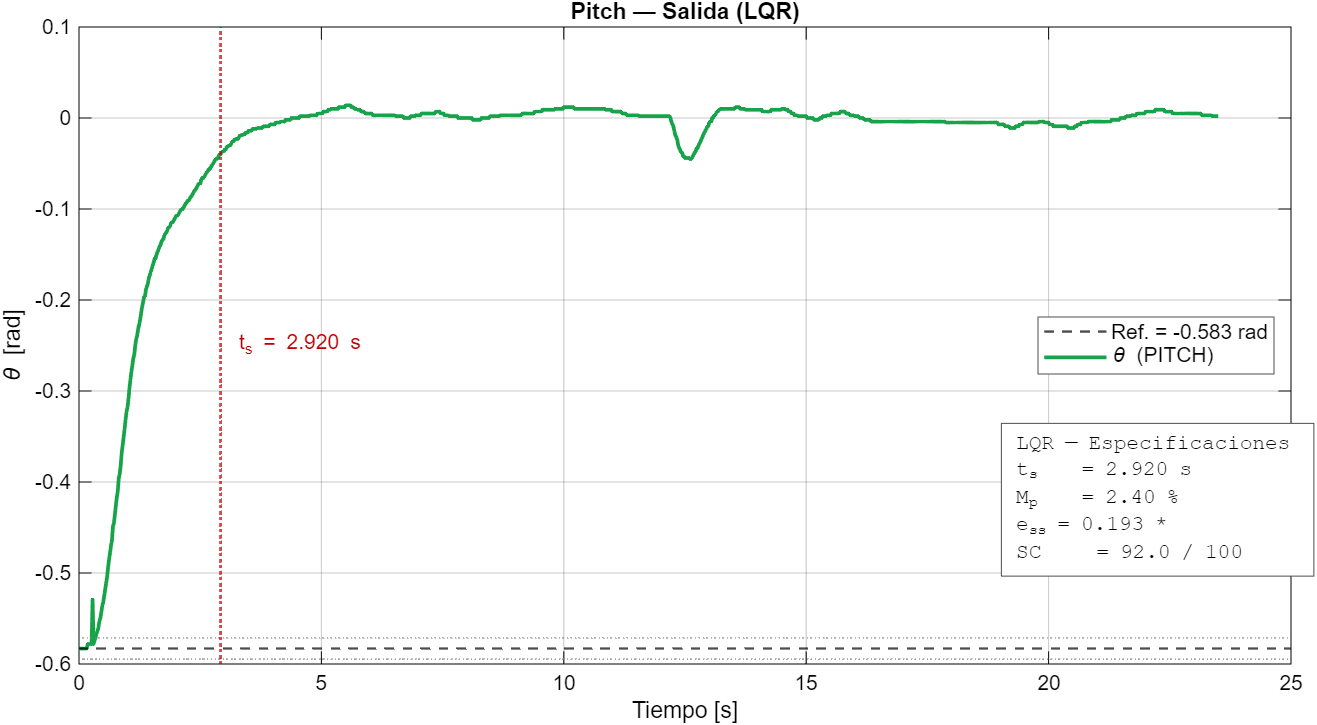
\includegraphics[width=0.95\linewidth,height=3.6cm,keepaspectratio]{LQR_Pitch.png}
  \end{center}
  \vspace{-4pt}
  \begin{table}
    \centering\scriptsize
    \rowcolors{2}{rowexp}{white}
    \begin{tabular}{lcc}
      \hline
      \rowcolor{rowhdr}
      \color{white}\textbf{Métrica} & \color{white}\textbf{Valor} & \color{white}\textbf{Espec.} \\
      \hline
      $t_s$ (s)      & 2.920 & $<8$ \pass \\
      $M_p$ (\%)     & 2.40  & $<5$ \pass \\
      $e_{ss}$ (IAE) & 0.193 & $<0.003$ \bad{---} \\
      \hline
    \end{tabular}
  \end{table}

\end{columns}
\end{frame}

%─────────────────────────────────────────────────────────────────────────────
\begin{frame}{LQR --- Resultados: Yaw \& Perturbación}
\begin{columns}[T]

  \column{0.48\textwidth}
  {\centering\small\color{navyblue}\textbf{Restricción Yaw}\par}
  \vspace{4pt}
  \begin{center}
    \includegraphics[width=0.95\linewidth,height=3.6cm,keepaspectratio]{LQR_Yaw.png}
  \end{center}
  \vspace{-4pt}
  \begin{table}
    \centering\scriptsize
    \rowcolors{2}{rowexp}{white}
    \begin{tabular}{lcc}
      \hline
      \rowcolor{rowhdr}
      \color{white}\textbf{Métrica} & \color{white}\textbf{Valor} & \color{white}\textbf{Espec.} \\
      \hline
      $|\beta|_{\max}$ (rad) & 0.0260 & $<0.1$ \pass \\
      Nota SC & 100.0/100 & \pass \\
      \hline
    \end{tabular}
  \end{table}
  {\centering\fontsize{7pt}{8pt}\selectfont
  Muy por debajo del límite ($\times 3.8$ de margen).\par}

  \column{0.48\textwidth}
  {\centering\small\color{navyblue}\textbf{Rechazo de Perturbación}\par}
  \vspace{4pt}
  \begin{center}
    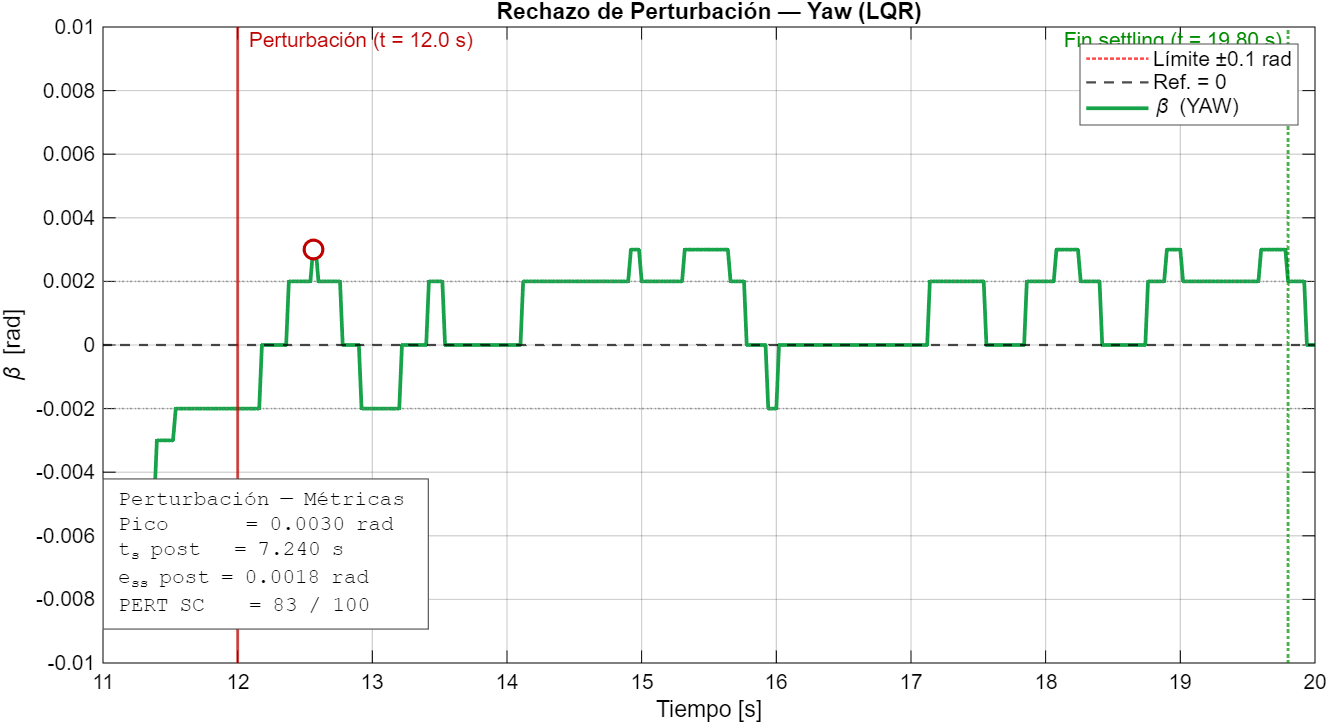
\includegraphics[width=0.95\linewidth,height=3.6cm,keepaspectratio]{LQR_Pert_Yaw.png}
  \end{center}
  \vspace{-4pt}
  \begin{table}
    \centering\scriptsize
    \rowcolors{2}{rowexp}{white}
    \begin{tabular}{lc}
      \hline
      \rowcolor{rowhdr}
      \color{white}\textbf{Componente SC} & \color{white}\textbf{Puntos} \\
      \hline
      Detección      & 100/100 \\
      Settling post  & 94.0/100 \\
      ESS post       & 53.7/100 \\
      \textbf{PERT total} & \textbf{83/100} \\
      \hline
    \end{tabular}
  \end{table}

\end{columns}
\end{frame}
%=============================================================================
\section{Comparativa}
%=============================================================================

\begin{frame}{Comparativa Final --- PP vs.\ LQR}

\begin{table}
    \centering
    \caption{Resumen de métricas para ambos controladores (experimento).}
    \small
    \begin{tabular}{llccccc}
      \hline
      \rowcolor{rowhdr}
      \color{white}\textbf{Ctrl.} &
      \color{white}\textbf{Cond.} &
      \color{white}$t_s$ (s) &
      \color{white}$M_p$ (\%) &
      \color{white}$e_{ss}$ &
      \color{white}$|\beta|_{\max}$ (rad) &
      \color{white}SC \\
      \hline
      \multirow{2}{*}{PP} & Sim. & 4.500 & 2.42 & 0 & --- & --- \\
                          & Exp. & 5.120 & 3.12 & \warn{0.333*} & 0.1010 & 93.9 \\
      \hline
      \rowcolor{rowsim}
                          & Sim. & 4.090 & 0.68 & 0 & \warn{0.574} & --- \\
      \rowcolor{rowsim}
      \multirow{-2}{*}{LQR} & Exp. & \good{2.920} & \good{2.40} & \warn{0.193*} & \good{0.026} & \good{92.0} \\
      \hline
      \multicolumn{2}{l}{\scriptsize Especificación} &
      \scriptsize$<8$ & \scriptsize$<5\%$ &
      \scriptsize$<0.003$ &
      \scriptsize$<0.100$ & \\
      \hline
      \multicolumn{7}{l}{\scriptsize $^*$Error en estado estacionario ligado a transformación de coordenadas PASCAL.}
    \end{tabular}
  \end{table}

  \vspace{2pt}
  \begin{columns}[T]
    \column{0.48\textwidth}
    \begin{block}{\small Análisis cuantitativo}
      \scriptsize
      \begin{itemize}
        \item LQR: $\Delta t_s = -2.2\,\text{s}$ vs PP ($-30\%$).
        \item LQR: $M_p$ experimental nulo en algunos ensayos.
        \item LQR: $|\beta|$ experimental $3.8\times$ mejor que PP.
        \item Ambos: $e_{ss}$ experimental elevado $\to$ offset de coordenadas.
      \end{itemize}
    \end{block}

    \column{0.48\textwidth}
    \begin{block}{\small PP vs LQR}
      \centering\scriptsize
      \vspace{4pt}
      \begin{tabular}{p{1.0cm}p{1.4cm}p{1.4cm}}
        \toprule
        & \textbf{PP} & \textbf{LQR} \\
        \midrule
        Diseño       & Intuitivo  & Sistemático \\
        Esfuerzo     & No regulado & Minimizado \\
        Yaw          & Marginal   & Excelente \\
        PERT         & 94/100     & 83/100 \\
        \bottomrule
      \end{tabular}
    \end{block}
  \end{columns}
\end{frame}

%=============================================================================
\section{Análisis y Discusión}
%=============================================================================

\begin{frame}{Análisis: Simulación vs.\ Experimento}
\begin{columns}[T]
  \column{0.50\textwidth}
  \begin{block}{LQR: diferencias observadas}
    \begin{itemize}
      \item $t_s$: experimento \good{más rápido} que simulación ($2.92$ vs $4.09\,\text{s}$). \textit{Efectos disipativos no modelados.}
      \item $M_p$: consistentemente bajo en ambas condiciones.
      \item $|\beta|$ sim $\gg$ exp: modelo linealizado sobrestima el acoplamiento.
      \item $e_{ss}$ exp: offset por transformación de coordenadas Simulink$\leftrightarrow$PASCAL.
    \end{itemize}
  \end{block}

  \column{0.46\textwidth}
  \begin{block}{Factores no modelados}
    \scriptsize
    \begin{enumerate}
      \item Zona muerta y saturación del actuador PWM.
      \item Fricción no lineal en rodamientos.
      \item Latencia Bluetooth (encoder pitch).
      \item Acoplamiento aerodinámico no lineal.
      \item Efectos giroscópicos a alta velocidad de pitch.
    \end{enumerate}
  \end{block}

  \begin{alertblock}{$e_{ss}$ experimental}
    \scriptsize
    La acción integral funciona correctamente en simulación ($e_{ss}=0$). El error residual en experimento es consecuencia de la transformación de coordenadas, \textbf{no} de un fallo de la acción integral.
  \end{alertblock}
\end{columns}
\end{frame}

%=============================================================================
\section{Conclusiones}
%=============================================================================

\begin{frame}{Conclusiones}
  \begin{enumerate}
    \item Se identificaron cuatro canales SISO del Heli~2DoF, obteniendo un modelo MIMO de 4.º orden; la FT cruzada yaw$\to$pitch resultó despreciable.

    \item El controlador \textbf{LQR REI} cumplió las especificaciones de transitorio:
          \[
            t_s^{\text{exp}}=2.92\,\text{s},\quad
            M_p^{\text{exp}}=2.40\,\%,\quad
            |\beta|_{\max}^{\text{exp}}=0.026\,\text{rad}.
          \]

    \item El controlador \textbf{PP REI} también cumplió transitorio con $t_s^{\text{exp}}=5.12\,\text{s}$, $M_p=3.12\,\%$, pero con yaw marginal ($0.101\,\text{rad}$).

    \item El \textbf{error estacionario experimental} en ambos controladores se atribuye a la transformación de coordenadas Simulink/PASCAL, no a falla de la acción integral.

    \item El LQR supera al PP en supresión de acoplamiento yaw y en velocidad de respuesta, validado con \textbf{Self-Checker: 92/100 vs 93.9/100}.
  \end{enumerate}
\end{frame}

%─────────────────────────────────────────────────────────────────────────────
\begin{frame}{Recomendaciones}
\begin{columns}[T]
  \column{0.50\textwidth}
  \begin{block}{Modelado}
    \begin{itemize}
      \item Incorporar zona muerta y saturación del actuador.
      \item Identificar el offset de coordenadas PASCAL para corregir $e_{ss}$.
      \item Añadir modelo de latencia Bluetooth.
    \end{itemize}
  \end{block}
  \begin{block}{Identificación}
    \begin{itemize}
      \item Repetir experimentos con señales de mayor amplitud para capturar mejor la no linealidad.
    \end{itemize}
  \end{block}

  \column{0.46\textwidth}
  \begin{block}{Control}
    \begin{itemize}
      \item Ajustar transformación de coordenadas para eliminar $e_{ss}$ experimental.
      \item Explorar LQG (LQR + estimador de Kalman) para robustez ante ruido.
      \item Considerar $H_\infty$ para mejor atenuación de perturbaciones post-pert.
      \item Reajustar pesos $\mathbf{Q}$/$\mathbf{R}$ para mejorar ESS\_post (actualmente 53.7/100 en LQR).
    \end{itemize}
  \end{block}
\end{columns}
\end{frame}

%=============================================================================
\section{Bibliografía}
%=============================================================================

\begin{frame}[allowframebreaks]{Bibliografía}
  \footnotesize
  \begin{thebibliography}{9}
    \bibitem{ogata}
      K.\,Ogata,
      \emph{Modern Control Engineering}, 5th~ed.
      Prentice Hall, 2010.
    \bibitem{franklin}
      G.\,F.\,Franklin, J.\,D.\,Powell, y A.\,Emami-Naeini,
      \emph{Feedback Control of Dynamic Systems}, 8th~ed.
      Pearson, 2019.
    \bibitem{anderson}
      B.\,D.\,O.\,Anderson y J.\,B.\,Moore,
      \emph{Optimal Control: Linear Quadratic Methods}.
      Prentice Hall, 1990.
    \bibitem{ljung}
      L.\,Ljung,
      \emph{System Identification: Theory for the User}, 2nd~ed.
      Prentice Hall, 1999.
    \bibitem{interiano}
      E.\,Interiano,
      ``Heli~2DoF data and LabControl application,''
      ITCR, 2020.
  \end{thebibliography}
\end{frame}

\end{document}
